\documentclass[8pt,a4paper,landscape]{article}
\usepackage[utf8]{inputenc}
\usepackage[english]{babel}
\usepackage{amsmath}
\usepackage{amsfonts}
\usepackage{amsthm}
\usepackage{amssymb}
\usepackage{graphicx}
\usepackage{float}
\usepackage[left=0.75cm,right=0.75cm,top=0.75cm,bottom=1.4cm]{geometry}
\usepackage[skins]{tcolorbox}
\usepackage{multicol}
\usepackage{calrsfs}
\usepackage{xcolor}
\usepackage{csquotes}
\usepackage{mathtools}
\usepackage{hyperref}
\usepackage{enumitem}


\definecolor{DarkGreen}{RGB}{1,100,32}

\setlength{\columnseprule}{1pt}

% Redefine the 'definition' style to have italic text
\newtheoremstyle{definition}      % Name (must match the one you're overriding)
  {\topsep}                       % Space above
  {\topsep}                       % Space below
  {\normalfont}                      % Body font -> italic
  {}                              % Indent amount
  {\bfseries}                     % Theorem head font
  {.}                             % Punctuation after theorem head
  { }                             % Space after theorem head
  {}                              % Theorem head spec
\theoremstyle{definition}
\newtheorem{definition}{Def.}[section]

\newtheoremstyle{example}      % Name of style
  {\topsep}                           % Space above
  {\topsep}                           % Space below
  {\itshape}                       % Body font (non-italic)
  {}                                  % Indent amount
  {\bfseries}                         % Theorem head font
  {.}                                 % Punctuation after theorem head
  { }                                 % Space after theorem head
  {}                                  % Theorem head spec
\theoremstyle{example}
\newtheorem{example}{Ex.}[section]

% Custom theorem style: intuition
\newtheoremstyle{intuition}    % Name
  {\topsep}                       % Space above
  {\topsep}                       % Space below
  {\color{DarkGreen}\normalfont}                   % Body font -> upright
  {}                              % Indent amount
  {\color{black}\bfseries}    % Theorem head font
  {.}                             % Punctuation after theorem head
  { }                             % Space after theorem head
  {}                              % Theorem head spec
\theoremstyle{intuition}
\newtheorem*{intuition}{Int}

\theoremstyle{definition}
\newtheorem{proposition}{Prop}[section]

\DeclareMathAlphabet{\pazocal}{OMS}{zplm}{m}{n}
%\newcommand{\La}{\mathcal{L}}
\newcommand{\Lb}{\pazocal{L}}
%\newcommand{\Fa}{\mathcal{F}}
\newcommand{\Fb}{\pazocal{F}}
\newcommand{\Pb}{\pazocal{P}}
\newcommand{\Ub}{\pazocal{U}}
\newcommand{\Cb}{\pazocal{C}}
\newcommand{\Nb}{\pazocal{N}}

\newcommand{\mydef}[1]{\textcolor{magenta}{\textbf{#1}}}
\newcommand{\prob}[1]{\mathbb{P}\left[ #1 \right]}
\newcommand{\expec}[1]{\mathbb{E}\left[ #1 \right]}

\DeclarePairedDelimiter\abs{\lvert}{\rvert}%
\DeclarePairedDelimiter\norm{\lVert}{\rVert}%

\MakeOuterQuote{"}



\author{Marc-Olivier Jufer \\ \href{mailto:mjufer@ethz.ch}{mjufer@ethz.ch}}
\title{Cheatsheet Probability and Statistics}


\begin{document}
\begin{multicols}{3}
	\maketitle
	
	
	\section{Mathematical framework}
			\subsection{Probability space}
			
			
				%sample space, outcome, elementary experiment
				\begin{definition}
					The set $\Omega$ is called the \mydef{sample space}. An element $\omega \in \Omega$ is called an \mydef{outcome} or \mydef{elementary experiment}.
				\end{definition}
				\begin{example}
					Throw of a die : $\Omega = \{1,2,3,4,5,6\}$
				\end{example}
				
				
				% sigma-algebra
				\begin{definition} \label{dsa}
					A \mydef{sigma-algebra} is a subset $\Fb \subset \Pb (\Omega)$ satisfying the following properties :
					\begin{description}
						\item[P1.] $\Omega \in \Fb$
						\item[P2.] $A \in \Fb \Rightarrow A^c \in \Fb$ : \textcolor{DarkGreen}{If $A$ is an event, "not $A$" is also an event.}
						\item[P3.] $A_1, A_2, \ldots \in \Fb \Rightarrow \bigcup\limits_{i=1}^{\infty}A_i \in \Fb$ : \textcolor{DarkGreen}{if $A_1, A_2, \ldots$ are events, then "$A_1$ or $A_2$ or $\ldots$" is an event}
					\end{description}
				\end{definition}
				\begin{example}
					Examples of sigma-algebras for $\Omega = \{1,2,3,4,5,6\}$ :
					\begin{itemize}
						\item $\Fb = \{\emptyset, \{1,2,3,4,5,6\}\}$
						\item $\Fb = \Pb(\Omega)$
						\item $\Fb = \{\emptyset, \{1,2\}, \{3,4,5,6\}, \{1,2,3,4,5,6\}\}$
					\end{itemize}
					Non examples of sigma-algebras for $\Omega = \{1,2,3,4,5,6\}$ :
					\begin{itemize}
						\item $\Fb  = \{\{1,2,3,4,5,6\}\}$ : \textbf{P2} is not satisfied
						\item $\Fb = \{\emptyset, \{1,2,3\},\{4,5,6\},\{1\},\{2,3,4,5,6\},\Omega\}$ : \textbf{P3} is not satisfied
					\end{itemize}
				\end{example}
				
				
				% probability measure
				\begin{definition} \label{dpm}
					Let $\Omega$ a sample space and $\Fb$ a sigma-algebra. A \mydef{probability measure} on $(\Omega, \Fb)$ is a map
					$$
						\mathbb{P}: \Fb \to \left[0,1\right], \quad A \mapsto \mathbb{P}\left[A\right] 
					$$
					that satisfies the properties
					\begin{description} 
						\item[P1.] $\mathbb{P}[\Omega] = 1$
						\item[P2. (countable additivity)] $\mathbb{P}[A] = \sum_{i=1}^{\infty} \mathbb{P}[A_i]$ if $A = \bigcup_{i=1}^{\infty} A_i$ (disjoint union)
					\end{description}
				\end{definition}
				\begin{intuition}
					A probability measure is a map that associates to each event a number in $[0,1]$
				\end{intuition}
				\begin{example}
					For $\Omega = \{1,2,3,4,5,6\}$ and $\Fb = \Pb(\Omega)$, the mapping $\mathbb{P}: \Fb \to [0,1]$ defined by 
					$$
						\forall A \in \Fb \quad \mathbb{P}[A] = \frac{\abs{A}}{6}
					$$
					is a probability measure on $(\Omega, \Fb)$.
				\end{example}
				
				
				% probability space
				\begin{definition}
					Let $\Omega$ a sample space, $\Fb$ a sigma-algebra and $\mathbb{P}$ a probability measure. The triple $(\Omega, \Fb, \mathbb{P})$ is called a \mydef{probability space}.
				\end{definition}
				
				
				% summary mathematical framework
				\begin{intuition}
					To construct a probabilistic model, we give
					\begin{itemize}
						\item a sample space $\Omega$ : all the possible outcomes of the experiment
						\item a sigma-algebra $\Fb \subset \Pb(\Omega)$ : the set of events
						\item a probability measure $\mathbb{P}$ : gives a number in $[0,1]$ to every event
					\end{itemize}
				\end{intuition}
				
				
				% occurs
				\begin{definition}
					Let $\omega \in \Omega$ (a possible outcome). Let $A$ be an event. We say the event $A$ \mydef{occurs} (\mydef{does not occur}) (for $\omega$) if $\omega \in A$ ($\omega \notin A$).
				\end{definition}
				
				
				
			\subsection{Examples of probability spaces}
			
				\begin{definition}
					Let $\Omega$ be a finite sample space. The \mydef{Laplace model} on $\Omega$ is the triple $(\Omega,\Fb, \mathbb{P})$, where $\Fb = \Pb(\Omega)$ and $\mathbb{P}: \Fb \to \left[0,1\right]$ is defined by
						$$
							\forall A \in \Fb \quad P\left[ A \right] = \frac{\abs{A}}{\abs{\Omega}}
						$$
				\end{definition}
				
				
			\subsection{Properties of Events}
				
				\begin{proposition}
					(Consequences of definition \ref{dsa}). Let $\Fb$ be a sigma-algebra on $\Omega$. We have
					\begin{description} 
						\item[P4.]  $\emptyset \in \Fb$
						\item[P5.] $A_1, A_2, \ldots \in \Fb \Rightarrow \bigcap_{i=1}^{\infty}A_i \in \Fb$
						\item[P6.] $A,B \in \Fb \Rightarrow A \cup B \in \Fb$
						\item[P7.] $A,B \in \Fb \Rightarrow A \cap B \in \Fb$
					\end{description}
				\end{proposition}
				
				\begin{figure}[H]
					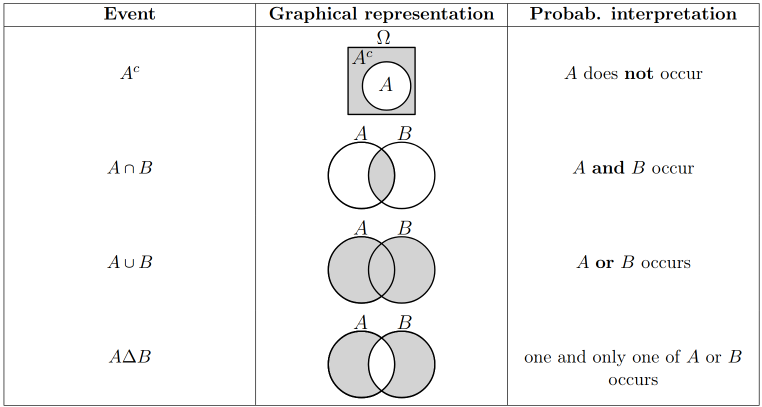
\includegraphics[width=\linewidth]{set-operations-representation.png}
					\caption{Representation of set operations}
				\end{figure}
				
%				Other set relations probabilistic interpretation :
%				\begin{itemize}
%					\item $A \subset B$ : If $A$ occurs, then $B$ occurs
%					\item $A \cap B = \emptyset$ : $A$ and $B$ cannot occur at the same time
%					\item $\Omega = A_1 \cup A_2 \cup A_3$ with $A_1,A_2,A_3$ pairwise disjoint : for each outcome $\omega$, one and only on of the events $A_1, A_2, A_3$ is satisfied.
%				\end{itemize}
				
				\begin{figure}[H]
					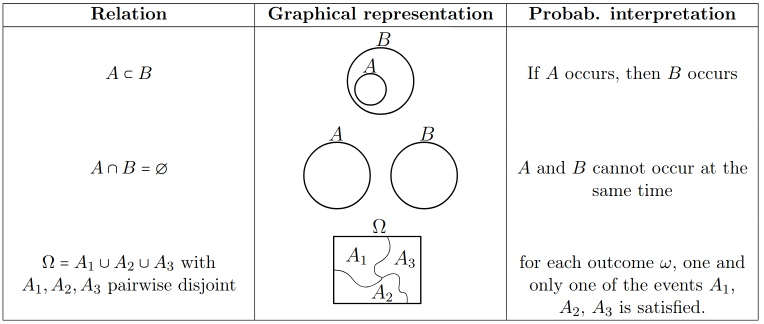
\includegraphics[width=\linewidth]{set-relations-representation.png}
					\caption{Representation of set relations}
				\end{figure}
				
				
			\subsection{Properties of probability measures}
			
				\begin{proposition}	
					(Consequences of definition \ref{dpm}). Let $\mathbb{P}$ be a probability measure on $(\Omega, \Fb)$.
					\begin{description}
						\item[P3.] We have $\mathbb{P}\left[\emptyset\right] = 0$
						\item[P4.] (\mydef{additivity}) Let $k \geq 1$, let $A_1, \ldots , A_k$ be $k$ pairwise disjoint events, then 
							$$
								\mathbb{P}\left[A_1 \cup \ldots \cup A_k \right] = \prob{A_1} + \ldots + \mathbb{P}\left[ A_k \right]
							$$
						\item[P5.] Let $A$ be an event, then
							$$
								\prob{A^c} = 1 - \prob{A}
							$$
						\item[P6.] If $A$ and $B$ are two events (not necessarily disjoint), then 
							$$
								\prob{A \cup B} = \prob{A} + \prob{B} - \prob{A \cap B}
							$$
					\end{description}
				\end{proposition}
				
				\begin{proposition}
					(\mydef{Monotonicity}). Let $A, B \in \Fb$, then
					$$
						A \subset B \Rightarrow \prob{A} \leq \prob{B}
					$$
				\end{proposition}
				
				\begin{proposition}
					(\mydef{Union bound}).Let $A_1, A_2, \ldots$ be a sequence of events (not necessarily disjoint), then we have
					$$
						\prob{\bigcup\limits_{i=1}^{\infty} A_i} \leq \sum_{i=1}^{\infty}\prob{A_i}
					$$
					Union bound also applies to a finite collection of events.
				\end{proposition}
				
				\begin{proposition}
					Let $(A_n)$ be an increasing sequence of events (i.e. $\forall n \ A_n \subset A_{n+1}$). Then
					\begin{center}
						$\lim_{n \rightarrow \infty} \prob{A_n} = \prob{\bigcup\limits_{n=1}{\infty} A_n}$. \mydef{increasing limit}
					\end{center}
					Let $(B_n)$ be a decreasing sequence of events (i.e. $\forall n \ B_n \supset B_{n+1}$). Then
					\begin{center}
						$\lim_{n \rightarrow \infty} \prob{B_n} = \prob{\bigcap\limits_{n=1}{\infty} B_n}$. \mydef{decreasing limit}
					\end{center}
				\end{proposition}
				
				
			\subsection{Conditional probabilities}
			
				% Conditional probabilitiy
				\begin{definition}
					Let $(\Omega, \Fb, \mathbb{P})$ be some probability space. Let $A, B$ be two events with $\prob{B} > 0$. The \mydef{conditional probability of} $A$ \mydef{given} $B$ is defined by
					$$
						\prob{A \lvert B} = \frac{A \cap B}{B}
					$$
				\end{definition}
				
				\begin{example}
					We consider the probability space $(\Omega, \Fb, \mathbb{P})$ corresponding to the throw of one die. Let $A = \{1,2,3\}$ and $B = \{2,4,6\}$. Then
					$$
						\prob{A \lvert B} = \frac{\prob{A \cap B}}{\prob{B}} = \frac{\frac{1}{6}}{\frac{1}{2}} = \frac{1}{3}
					$$
				\end{example}
				
				\begin{proposition}
					Let $(\Omega, \Fb, \mathbb{P})$ be some probability space. Let $B$ be an event with positive probability. Then $\prob{\ . \ \lvert B}$ is a probability measure on $\Omega$.
				\end{proposition}
				
				% Total probability
				\begin{proposition}
					(\mydef{Formula of total probability}). Let $B_1, \ldots, B_n$ be a partition\footnote{i.e. $\Omega = B_1 \cup \ldots \cup B_n$ and the events are pairwise disjoint.} of the sample space $\Omega$ with $\prob{B_i} > 0$ for every $i \leq i \leq n$. Then one has
					$$
						\forall A \in \Fb \quad \prob{A} = \sum_{i=1}^n \prob{A \lvert B_i} \prob{B_i}
					$$
				\end{proposition}
				
				% Bayes formula
				\begin{proposition}
					(\mydef{Bayes formula}). Let $B_1, \ldots, B_n \in \Fb$ be a partition of $\Omega$ with $\prob{B_i} > 0 \ \forall i$. For every event $A$ with $\prob{A} > 0$ we have 
					$$
						\forall i = 1, \ldots, n \quad \prob{B_i \lvert A} = \frac{\prob{A \vert B_i} \prob{B_i}}{\sum_{j=1}^n \prob{A \lvert B_j} \prob{B_j}}
					$$
				\end{proposition}
				
				\begin{example}
					Test to detect a disease which concerns about $1/10000$ of the population. The test gives the right answer $99\%$ of the time. If a patient has a positive test, what is the probability that he is actually sick ?\\
					We modeled the situation as $\Omega = \{0,1\} \times \{0,1\}$. $\Fb = \Pb(\Omega)$ and an outcome is $\omega = (\omega_1, \omega_2)$, where $\omega_1$ is $1$ if the patient is sick and $\omega_2$ is $1$ if the test is positive. Let $S = \{(1,0), (1,1)\}$ be the event that the patient is sick and $T = \{(0,1),(1,1)\}$ the event that the test is positive.\\
					From the hypotheses, we have
					$$
						\prob{S} = \frac{1}{10000}, \quad \prob{T \lvert S} = \frac{99}{100}, \quad \prob{T \lvert S^c} = \frac{1}{100}
					$$
					By applying the Bayes formula to the partition $\Omega = S \cup S^c$, we obtain
					$$
						\prob{S \lvert T} = \frac{\prob{T \lvert S} \prob{S}}{\prob{T \lvert S} \prob{S} + \prob{T \lvert S^c} \prob{S^c}} \simeq 0.0098
					$$
				\end{example}
				
				
			\subsection{Independence}
			
				% Independence of events
				\begin{definition}
					Let $(\Omega, \Fb, \mathbb{P})$ be a probability space. Two events $A$ and $B$ are said to be \mydef{independent} if 
					$$
						\prob{A \cap B} = \prob{A} \prob{B}
					$$
					$A$ is independent of $B$ iff $A$ is independent of $B^c$. \\
					If $\prob{A} \in \{0,1\}$, then $A$ is independent of every event. \\
					If $A$ is independent with itself (i.e. $\prob{A \cap A} = \prob{A}^2$), then $\prob{A} \in \{0, 1\}$.
				\end{definition}
				
				\begin{proposition}
					Let $A, B \in \Fb$ be two events with $\prob{A}, \prob{B} > 0$. Then the following are equivalent :
					\begin{enumerate}[label=\roman*.]
						\item $\prob{A \cap B} = \prob{A} \prob{B}$ : \textcolor{DarkGreen}{A and B are independent}
						\item $\prob{A \lvert B} = \prob{A}$ : \textcolor{DarkGreen}{the occurrence of B has no influence on A}
						\item $\prob{B \lvert A} = \prob{B}$ : \textcolor{DarkGreen}{the occurrence of A has no influence on B}
					\end{enumerate} 
				\end{proposition}
				
				% Independence of collection of events
				\begin{definition}
					Let $I$ be an arbitrary set of indices. A collection of events $(A_i)_{i \in I}$ is said to be \mydef{independent} if 
					$$
						\forall J \subset I finite \quad \prob{\bigcap\limits_{j \in J} A_j} = \prod_{j \in J} \prob{A_j}
					$$
				\end{definition}
				
				\begin{intuition}
					Three events $A$, $B$ and $C$ are independent if the following 4 equations are satisfied :
						$$\prob{A \cap B} = \prob{A} \prob{B} $$
						$$\prob{A \cap C} = \prob{A} \prob{C} $$
						$$\prob{B \cap C} = \prob{B} \prob{C} $$
						$$\prob{A \cap B \cap C} = \prob{A}\prob{B}\prob{C}$$
				\end{intuition}


	\newpage
	\section{Random variables and distribution functions}
			\subsection{Abstract definition}
			
				% Random variable
				\begin{definition}
					Let $(\Omega, \Fb, \mathbb{P})$ be a probability space. A \mydef{random variable} (r.v.) is a map $X : \Omega \to \mathbb{R}$ s.t.
					$$						
						\forall a \in \mathbb{R} \quad \{\omega \in \Omega : X(\omega) \leq a\} \in \Fb
					$$
				\end{definition}
				
				\begin{example}
					We throw a fair die. The sample space is $\Omega = \{1,2,3,4,5,6\}$ and we consider the Laplace model $(\Omega, \Fb, \mathbb{P})$. Suppose we gamble on the outcome in such a way that our profit is $-1$ if the outcome is $1$, $2$ or $3$ ; $0$ if the outcome is $4$ and $2$ if the outcome is $5$ or $6$. Our profit can be represented by the mapping $X$ defined by 
					$$
						\forall \omega \in \Omega \quad X(\omega) = \begin{cases}
							-1 \quad \text{if } \omega = 1,2,3, \\
							0 \quad \text{if } \omega = 4, \\
							2 \quad \text{if } \omega = 5,6
						\end{cases}
					$$
					Since $\Fb = \Pb(\Omega)$, we have $\{\omega : X(\omega) \leq a\} \in \Fb$ for every $a$. Therefore, $X$ is a random variable on $(\Omega, \Fb, \mathbb{P})$.
				\end{example}
				
				\begin{definition}
					When events are defined in terms of random variable, we omit the dependence in $\omega$. E.g. for $a \leq b$ we write 
					$$\{X \leq a\} = \{\omega \in \Omega : X(\omega) \leq a\}$$
					$$\{a < X \leq b\} = \{\omega \in \Omega : a < X(\omega) < b\}$$
					$$\{X \in \mathbb{Z}\} = \{\omega \in \Omega : X(\omega) \in \mathbb{Z}\}$$
					When consider the probability of events as above, we omit the brackets 
					$$ \prob{X \leq a} = \prob{\{X \leq a\}} = \prob{\{\omega \in \Omega : X(\omega) \leq a\}}$$
				\end{definition}
				
			
			\subsection{Distribution function}
			
				% Distribution function
				\begin{definition}
					Let $X$ be a random variable on a prob. space $(\Omega, \Fb, \mathbb{P})$. The \mydef{distribution function of X} is the function $F_X : \mathbb{R} \to \left[0,1\right]$ defined by
					$$
						\forall a \in \mathbb{R} \quad F_X(a) = \prob{X \leq a}
					$$
				\end{definition}
				
				\begin{example}
					Same example with the die. Let $X$ be the random variable defined as above. For $a \in \mathbb{R}$ we have 
					$$
						F_X(a) = \begin{cases}
							0 \quad \text{if } a < -1,\\
							1/2 \quad \text{if } -1 \leq a < 0, \\
							2/3 \quad \text{if } 0 \leq a < 2, \\
							1 \quad \text{if } a \geq 2
						\end{cases}
					$$
					\begin{figure}[H]
						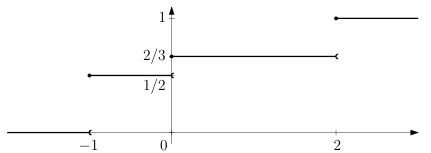
\includegraphics[width=\linewidth]{distribution_function.png}
						\caption{Graph of the distribution function $F_X$}
					\end{figure}
				 \end{example}
				 
				 \begin{proposition}
				 	(\mydef{Basic identity}). Let $a < b$ be two real numbers. Then 
				 	$$
				 		\prob{a < X \leq b} = F(b) - F(a)
				 	$$
				 \end{proposition}
				 
				 \begin{proposition} \label{FX-conditions}
				 	Let $X$ be a r.v. on some probability space $(\Omega, \Fb, \mathbb{P})$. The distribution function $F = F_X : \mathbb{R} \to \left[0,1\right]$ of $X$ satisfies the following properties :
					\begin{enumerate}[label=\roman*.] \label{F_3points}
				 		\item $F$ is nondecreasing
				 		\item $F$ is right continuous\footnote{i.e. $F(a) = \lim_{h \downarrow 0}F(a+h)$ for every $a \in \mathbb{R}$}
				 		\item $\lim\limits_{a \rightarrow -\infty} F(a) = 0$ and $\lim\limits_{a \rightarrow \infty} F(a) = 1$
				 	\end{enumerate}
				 \end{proposition}
				 
				 
			\subsection{Independence}
				
				% Independence of random variables
				\begin{definition}
					Let $X_1, \ldots, X_n$ be $n$ random variables on some probability space $(\Omega, \Fb, \mathbb{P})$. We say that they are \mydef{independent} if
					$
						\forall x_1, \ldots, x_n \in \mathbb{R} \quad \prob{X_1 \leq x_1, \ldots, X_n \leq x_n} 
						= \prob{X_1 \leq x_1} \ldots \prob{X_n \leq x_n}
					$.\\
					One can show that $X_1, \ldots, X_n$ are independent iff $\forall I_1 \subset \mathbb{R}, \ldots, I_n \subset \mathbb{R}$ intervals $\{X_1 \in I_1\}, \ldots, \{X_n \in I_n\}$ are independent.
				\end{definition}
				
				% Grouping
				\begin{proposition}
					(\mydef{Grouping}). Let $X_1, \ldots, X_n$ be $n$ independent r.v. Let $1 \leq i_1 < i_2 < \ldots < i_k \leq n$ be some indices and $\phi_1, \ldots, \phi_k$ some functions. Then 
					$Y_1 = \phi_1 (X_1, \ldots, X_{i_1}), Y_2 = \phi_2(X_{i_1 + 1}, \ldots, X_{i_2}), \ldots, Y_k = \phi_k (X_{i_{k-1}+1}, \ldots, X_{i_k})$
					are independent.
				\end{proposition}
				
				% Sequences of i.i.d. random variables
				\begin{definition}
					An infinite sequence $X_1, X_2, \ldots$ of random variables is said to be 
					\begin{itemize}
						\item \mydef{independent} if $X_1, \ldots, X_n$ are independent for every $n$
						\item \mydef{independent and identically distributed} (i.i.d) if they are independent and they have the same distribution function, i.e. $\forall i,j \quad F_{X_i} = F_{X_j}$.
					\end{itemize}
				\end{definition}
				
				
			\subsection{Transformation of random variables}
				
				% peut-être commenter les deux premières lignes
				We can create r.v. from other r.v. on the same probability space. For example, consider $Z_1 = \exp(X_1), Z_2 = X_1 + X_2$. Not to forget : r.v. are maps $\Omega \to \mathbb{R}$.\\
				We can work with r.v. as if they were real numbers with the following notation :
				\begin{definition}
					If $X$ is a r.v. and $\phi : \mathbb{R} \to \mathbb{R}$, then we write 
					$$
						\phi(X) := \phi \circ X 
					$$
					to to $\phi(X)$ a new mapping $\Omega \to \mathbb{R}$.\\
					We also consider function of several variables. If $X_1, \ldots, X_n$ are $n$ r.v. and $\phi : \mathbb{R}^n \to \mathbb{R}$, then we write 
					$$
						\phi(X_1, \ldots, X_n) := \phi \circ (X_1, \ldots, X_n)
					$$
				\end{definition} 

			
			\subsection{Construction of random variables}
				
				% Bernoulli random variables
			\begin{definition} \label{Bernoulli_rv}
					Let $p \in \left[0,1\right]$. A r.v. $X$ is said to be a \mydef{Bernoulli r.v. with parameter $p$} if 
					$$
					\prob{X = 0} = 1-p \quad \text{and} \quad \prob{X = 1} = p
					$$
				In this case, we write $X \sim \text{Ber}(p)$.
				\end{definition}

				% Existence theorem of Kolmogorov
				\begin{proposition}
					(\mydef{Existence theorem of Kolmogorov}). There exists a probability space $(\Omega, \Fb, \mathbb{P})$ and an infinite sequence of r.v. $X_1, X_2, \ldots$ (on this probability space) that is an iid sequence of Bernoulli r.v. with parameter $1/2$.
				\end{proposition}

				% Uniform random variable
				\begin{proposition}
					A r.v. $U$ is said to be \mydef{uniform r.v. in $\left[0,1\right]$} if its distribution function is equal to 
					$$
					F_U(x) = \begin{cases}
						0 \quad x < 0 \\
						x \quad 0 \leq x \leq 1 \\
						1 \quad x > 1
					\end{cases}
					$$
					In this csae, we write $U \sim \Ub (\left[0,1\right])$.
				\end{proposition}

				% Distribution functions of benroulli and uniform random variables
				\begin{figure}[H] 
					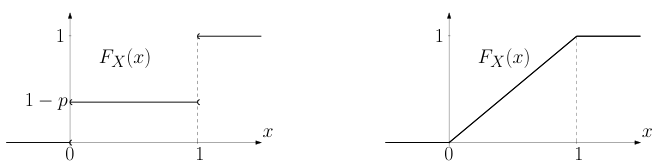
\includegraphics[width=\linewidth]{bernoulli_uniform_rv.png}
					\caption{Left: distribution function of a Bernoulli r.v. with parameter $p$. Right: distribution function of a uniform r.v. in $\left[0,1\right]$.}
				\end{figure}

				\begin{proposition}
					The mapping $Y : \Omega \to \left[0,1\right]$ defined by $Y(\omega) = \sum_{n=1}^{\infty}2^{-n}X_n(\omega)$ is a uniform r.v. in $\left[0,1\right]$.
				\end{proposition}

				% Generalized inverse
				\begin{definition}
					The \mydef{generalized inverse} of $F$\footnote{\label{note3}satifying prop. \ref{F_3points}} is the mapping $F^{-1} : (0,1) \to \mathbb{R}$ defined by
					$$
						\forall \alpha \in (0,1) \quad F^{-1}(\alpha) = \text{inf}\{x \in \mathbb{R} : F(x) \geq \alpha\}
					$$
				\end{definition}

				\begin{intuition}
					By definition of the infimum and using right continuity of $F$, we have $\forall x \in \mathbb{R}$ and $\forall \alpha \in (0,1)$
					$$
						(F^{-1}(\alpha) \leq x) \Longleftrightarrow (\alpha \leq F(x))
					$$
				\end{intuition}

				% Inverse transform sampling
				\begin{proposition}
					(\mydef{Inverse transform sampling}). Let $F : \mathbb{R} \to \left[0,1\right]$.\footnote{See footnote \ref{note3}} Let $U$ be a uniform r.v. in $\left[0,1\right]$. Then the r.v. $X = F^{-1}(U)$ has distribution $F_X = F$.
				\end{proposition}

				% General sequence of independent random variables
				\begin{proposition}
					Let $F_1, F_2, \ldots$ be a sequence of functions $\mathbb{R} \to \left[0,1\right]$.\footnote{See footnote \ref{note3}} Then there exist a probability space $(\Omega, \Fb, \mathbb{P})$ and a sequence of independent r.v. $X_1, X_2, \ldots$ on this probability space s.t.
					\begin{itemize}
						\item for every $i$ $X_i$ has distribution function $F_i$ (i.e. $\forall x \prob{X_1 \leq x} = F_i(x)$)
						\item $X_1, X_2, \ldots$ are independent
					\end{itemize}
				\end{proposition}


	\section{Discrete and continuous r.v.}
		\subsection{Discontinuity / continuity points of $F$}
			
			% Probability of a given value
			\begin{proposition}
				Let $X : \Omega \to \mathbb{R}$ be a r.v. with distribution function $F$. Then for every $a$ in $\mathbb{R}$ we have
				$$
					\prob{X = a} = F(a) - F(a-)
				$$
				where $F(a-) := \lim_{h \downarrow 0}F(a-h)$.
			\end{proposition}

			\begin{intuition}
				Fix $a \in \mathbb{R}$
				\begin{itemize}[label=$\rightarrow$]
					\item If $F$ is not continuous at a point $a \in \mathbb{R}$, then the "jump size" $F(a) - F(a-)$ is equal to the probability that $X = a$
					\item If $F$ is continuous at a point $a \in \mathbb{R}$, then $\prob{X = a} = 0$
				\end{itemize}
			\end{intuition}

	
		\subsection{Almost sure events}
			
			% almost surely
			\begin{definition}
				Let $A \in \Fb$ be an event. We say that $A$ occurs \mydef{almost surely} (\mydef{a.s.}) if $\prob{A} = 1$.
			\end{definition}

		
		\subsection{Discrete random variables}

			% Discrete random variables
			\begin{definition}
				A r.v. $X : \Omega \to \mathbb{R}$ is said to be \mydef{discrete} if there exists some set $W \subset \mathbb{R}$ finite or countable s.t. $X \in W \quad \text{a.s.}$.
			\end{definition}

			% Distribution of discrete random variables
			\begin{definition}
				Let X be a discrete r.v. taking some values in some finite or countable set $W \subset \mathbb{R}$. The \mydef{distribution of} $X$ is the sequence of numbers $(p(x))_{x \in W}$ defined by 
				$$
					\forall x \in W \quad p(x) := \prob{X = x}
				$$
			\end{definition}

			\begin{proposition}
				The distribution $(p(x))_{x \in W}$ of a discrete r.v. satisfies $\sum_{x \in W} p(x) = 1$.
			\end{proposition}

			\begin{proposition}
				Let $X$ be a discrete r.v. with values in a finite or countable set $W$ almost surely, and distribution $p$. Then the distribution function of $X$ is given by
				$$
				\forall x \in \mathbb{R} \quad F_X(x) = \sum_{\substack{y \leq x \\ y \in W}} p(y)
				$$
			\end{proposition}

			\begin{intuition}
				$W = \{\text{positions of the jumps of } F_X\}$,\\
				$p(x) = \text{"height of the jump" at } x \in W$.
			\end{intuition}


		\subsection{Examples of discrete random variables}
			
		 	The simplest (non constant) r.v. is the Bernoulli r.v. defined in definition \ref{Bernoulli_rv}.

			% Binomial distribution
			\begin{definition}
				Let $0 \leq p \leq 1$, let $n \in \mathbb{N}$. A r.v. $X$ is said to be a \mydef{binomial r.v. with parameters $n$ and $p$} if it takes values in $W = \{0,\ldots, n\}$ and 
				$$
				\forall k \in \{0,\ldots,n\} \quad \prob{X = k} = \binom{n}{k} p^k (1-p)^{n-k}
				$$
				In that case we write $X \sim \text{Bin}(n,p)$.
			\end{definition}

			% Sum of independent Bernoulli and binomial
			\begin{proposition}
				(\mydef{Sum of independent Bernoulli and binomail}. Let $0 \leq p \leq 1$, let $n \in \mathbb{N}$. Let $X_1, \ldots, X_n$ be $n$ independent Bernoulli r.v. with parameter $p$. Then
				$$
					S_n := X_1 + \ldots + X_n
				$$
				is a binomial r.v. with parameter $n$ and $p$.
			\end{proposition}

			\begin{intuition}
				In particular, the distribution $\text{Bin}(1,p)$ is the same as the distribution $\text{Ber}(p)$. On can also check that if $X \sim \text{Bin}(m,p)$ and $Y \sim \text{Bin}(n,p)$ and $X,Y$ are independent, then $X + Y \sim \text{Bin}(m + n, p)$.
			\end{intuition}

			% Geometric distribution
			\begin{definition}
				Let $0 \leq p \leq 1$. A r.v. $X$ is said to be a \mydef{geometric r.v. with parameter $p$} if it takes values in $W = \mathbb{N} \setminus \{0\}$ and 
				$$
					\forall k \in \mathbb{N} \quad \prob{X = k} = (1-p)^{k-1} \cdot p
				$$
				In this case, we write $X \sim \text{Geom}(p)$.
			\end{definition}

			% Geometric r.v. appears naturally as the first success in an infinite sequence of Bernoulli experiments with parameter p
			\begin{proposition}
				Let $X_1, X_2, \ldots$ be a sequence of infinitely many independent Bernoulli r.v. with parameter $p$. Then
				$$
				T := \min\{n \geq 1 : X_n = 1\}
				$$
				is a geometric r.v. with parameter $p$.
			\end{proposition}

			% Absence of memory of the geometric distribution
			\begin{proposition}
				(\mydef{Absence of memory of the geometric distribution}). Let $T \sim \text{Geom}(p)$ for some $0 < p < 1$. Then
				$$
					\forall n \geq 0 \ \forall k \geq 1 \quad \prob{T \geq n + k \lvert T > n} = \prob{T \geq k}
				$$
			\end{proposition}

			% Poisson distribution
			\begin{definition}
				Let $\lambda > 0$ be a positive real number. A r.v. $X$ is said to be a \mydef{Poisson r.v. with parameter $\lambda$} if it takes values in $W = \mathbb{N}$ and 
				$$
				\forall k \in \mathbb{N} \quad \prob{X = k} = \frac{\lambda^k}{k!} e^{-\lambda}
				$$
				In this case, we write $X \sim \text{Poisson}(\lambda)$.
			\end{definition}

			% Poisson distribution appears naturally as an approximation of a binomail distribution when the parameter n is large and the parameter p is small
			\begin{proposition}
				(\mydef{Poisson approximation of the binomail}). Let $\lambda > 0$. For every $n \geq 1$, consider a r.v. $X_n \sim \text{Bin}(n, \frac{\lambda}{n})$. Then
				$$
					\forall k \in \mathbb{N} \quad \lim\limits_{n \to \infty} \prob{X_n = k} = \prob{N = k}
				$$
				where $N$ is a Poisson r.v. with parameter $\lambda$.
			\end{proposition}


		\subsection{Continous random variables}
			
			% Continuous random variables
			\begin{definition}
				A r.v. $X : \Omega \to \mathbb{R}$ is said to be \mydef{continuous} if its distribution function $F_X$ can be written as
				$$
				F_X(a) = \int_{-\infty}^{a} f(x)\, dx \quad \text{for all } a \in \mathbb{R}
				$$
				for some nonnegative function $f : \mathbb{R} \to \mathbb{R_+}$, called the \mydef{density} of $X$.
			\end{definition}

			\begin{intuition}
				$f(x)\, dx$ represents the probability that $X$ takes a value in the infinitesimal interval $\left[x, x + dx\right]$.
			\end{intuition}

			\begin{proposition}
				The density $f$ of a r.v. satisfies $\int_{-\infty}^{+\infty} f(x)\, dx = 1$.
			\end{proposition}

			\begin{proposition}
				Let $X$ be a r.v. Assume the distribution function $F_X$ is continuous and piecewise $\Cb^1$, i.e. that there exist $x_0 = -\infty < x_1 < \ldots < x_{n-1} < x_n = +\infty$ s.t. $F_X$ is $\Cb^1$ on every interval $(x_i, x_{i+1}$. Then $X$ is a continuous r.v. and a density $f$ can be constructed by defining 
				$$
					\forall x \in (x_i, x_{i+1}) \quad f(x) = F'_X(x)
				$$
				and setting arbitrary values at $x_1, \ldots, x_{n-1}$.
			\end{proposition}


		\subsection{Examples of continuous random variables}
				
			% Uniform distribution in [a,b], a<b
			\begin{definition}
				A continuous r.v. $X$ is said to be \mydef{uniform in $\left[a,b\right]$} if its density is equal to 
				$$
					f_{a,b}(x) = \begin{cases}
						\frac{1}{b-a} \quad x \in \left[a,b\right], \\
						0 						\quad x \notin \left[a,b\right]
					\end{cases}
				$$
				In this case, we write $X \sim \Ub(\left[a,b\right])$.
			\end{definition}

			% Exponential distribution with \lambda > 0
			\begin{definition}
				A continuous r.v. $T$ is said to be \mydef{exponential with parameter $\lambda > 0$} if its density is equal to 
				$$
					f_\lambda(x) = \begin{cases}
						\lambda e^{-\lambda x} \quad x \geq 0, \\
						0 										 \quad x < 0
					\end{cases}
				$$
				In this case, we write $T \sim \text{Exp}(\lambda)$.
			\end{definition}

			% Normal distribution with parameters m and \sigma^2 > 0
			\begin{definition}
				A continuous r.v. $X$ is said to be \mydef{normal with parameters $m$ and $\sigma^2 > 0$} if its density is equal to 
				$$
					f_{m,\sigma}(x) = \frac{1}{\sqrt{2 \pi \sigma^2}} e^{\frac{(x-m)^2}{2 \sigma^2}}
				$$
				In this case, we write $X \sim \Nb(m,\sigma^2)$.
			\end{definition}


	\section{Expectation}
		\subsection{Expectation for general r.v.}
			\begin{definition}
				Let $X : \Omega \to \mathbb{R}_+$ be a r.v. with nonnegative values. The \mydef{expectation} of $X$ is defined as 
				$$
					\expec{X} = \int_0^\infty (1 - F_X(x)) dx
				$$
			\end{definition}

			\begin{proposition}
				Let $X$ be a nonnegative r.v. Then we have $\expec{X} \geq 0$, with equality iff $X=0$ almost surely.
			\end{proposition}

			\begin{definition}
				Let $X$ be a r.v. If $\expec{\lvert X \lvert} < \infty$, then the expectation of $X$ is defined by $\expec{X} = \expec{X_+} - \expec{X_-}$, where $X_+$ and $X_-$ are the positive and negative parts of $X$ defined by $X_+(\omega) = \begin{cases} X(\omega) \quad \text{if } X(\omega) \geq 0, \\ 0 \quad \text{if } X(\omega) < 0,\end{cases}$ and $X_-(\omega) = \begin{cases} -X(\omega) \quad \text{if } X(\omega) \leq 0, \\ 0 \quad \text{if } X(\omega) > 0.\end{cases}$
			\end{definition}


		\subsection{Expectation of a discrete r.v.}
			\begin{proposition}
				Let $X : \Omega \to \mathbb{R}$ be a discrete r.v. with values in $W$ (finite or countable) almost surely. We have
				$$
					\expec{X} = \sum_{x \in W} x \cdot \prob{X = x}
				$$
				provided the sum is well defined.
			\end{proposition}

			\begin{proposition}
				Let $X : \Omega \to \mathbb{R}$ be a discrete r.v. with values in $W$ (finite or countable) almost surely. For every $\phi : \mathbb{R} \to \mathbb{R}$, we have
				$$
					\expec{\phi(X)} = \sum_{x \in W} \phi(x) \cdot \prob{X = x}
				$$
				provided the sum is well defined.
			\end{proposition}


		\subsection{Expectation of a continuous r.v.}
			\begin{proposition}
				Let $X$ be a contiuous r.v. with density $f$. Then we have 
				$$
					\expec{X} = \int_{-\infty}^\infty x \cdot f(x) dx
				$$
				provided the integral is well defined.
			\end{proposition}

			\begin{proposition}
				Let $X$ be a continuous r.v. with density $f$. Let $\phi : \mathbb{R} \to \mathbb{R}$ be s.t. $\phi(X)$ is a r.v. Then we have
				$$
					\expec{\phi(X)} = \int_{-\infty}^\infty \phi(x) f(x) dx
				$$
				provided the integral is well defined.
			\end{proposition}


		\subsection{Calculus}
			\begin{proposition}
				(\mydef{Linearity of the expectation}). Let $X,Y : \Omega \to \mathbb{R}$ be r.v.'s, let $\lambda \in \mathbb{R}$. Provided the expectations are well defined, we have 
				\begin{enumerate}
					\item $\expec{\lambda \cdot X} = \lambda \cdot \expec{X}$
					\item $\expec{X + Y} = \expec{X} + \expec{Y}$
				\end{enumerate}
			\end{proposition}

			\begin{proposition}
				Let $X,Y$ be two r.v. If $X$ and $Y$ are independent, then $\expec{XY} = \expec{X} \expec{Y}$.
			\end{proposition}


		\subsection{Tailsum formulas}
			\begin{proposition}
				(\mydef{Tailsum formula for nonnegative r.v.'s}). Let $X$ be a r.v., s.t. $X \geq 0$ almost surely. Then we have $\expec{X} = \int_0^\infty \prob{X > x} dx$.
			\end{proposition}

			\begin{proposition}
				(\mydef{Tailsum formula for discrete r.v.'s}). Let $X$ be a discrete r.v. taking values in $\mathbb{N} = \{0,1,2,\ldots\}$. Then
				$
					\expec{X} = \sum_{n=1}^\infty \prob{X \geq n}
				$.
			\end{proposition}


		\subsection{Characterizations via expecations}
			\begin{proposition}
				Let $X$ be a r.v. Let $f : \mathbb{R} \to \mathbb{R}$ s.t. $\int_{-\infty}^{+\infty} f(x) dx = 1$. then the following are equivalent :
				\begin{enumerate}[label=\roman*.]
					\item $X$ is continuous with density $f$,
					\item For every function $\phi : \mathbb{R} \to \mathbb{R}$ piecwise continuous, bounded : $\expec{\phi(X)} = \int_{-\infty}^\infty \phi(x) f(x) dx$
				\end{enumerate}
			\end{proposition}

			\begin{proposition}
				Let $X,Y$ be two discrete r.v.'s. Then the following are equivalent 
				\begin{enumerate}[label=\roman*.]
					\item $X,Y$ are independent
					\item For every $\phi : \mathbb{R} \to \mathbb{R}$, $\psi : \mathbb{R} \to \mathbb{R}$ piecewise contiuous, bounded : $\expec{\phi(X)\psi(Y)} = \expec{\phi(X)} \expec{\psi(Y)}$.
				\end{enumerate}
			\end{proposition}

			\begin{proposition}
				Let $X_1, \ldots, X_n$ be $n$ r.v.'s. Then the following are equivalent
				\begin{enumerate}[label=\roman*.]
					\item $X_1, \ldots, X_n$ are independent
					\item For every $\phi_1 : \mathbb{R} \to \mathbb{R}, \ldots, \phi_n : \mathbb{R} \to \mathbb{R}$ piecewise continuous, bounded : $\expec{\phi_1(X_1) \cdots \phi_n(X_n)} = \expec{\phi_1(X_1)} \cdots \expec{\phi_n(X_n)}$.
				\end{enumerate}
			\end{proposition}


		\subsection{Inequalities}
			% Monotonicity
			\begin{proposition}
				(\mydef{Monotonicity}). Let $X,Y$ be two r.v.'s s.t. $X \leq Y$ a.s. Then
				$
					\expec{X} \leq \expec{Y}
				$,
				provided the two expectations are well defined.
			\end{proposition}

			% Markov's inequality
			\begin{proposition}
				(\mydef{Markov's inequality}). Let $X$ be a nonnegative r.v. Then for every $a > 0$, we have 
				$$
					\prob{X \geq a} \leq \frac{\expec{X}}{a}
				$$
			\end{proposition}

			% Jensen's inequality
			\begin{proposition}
				(\mydef{Jensen's inequality}). Let $X$ be a r.v. Let $\phi : \mathbb{R} \to \mathbb{R}$ be a convex function. If $\expec{\phi(X)}$ and $\expec{X}$ are well defined, then
				$$
					\phi(\expec{X}) \leq \expec{\phi(X)}
				$$
			\end{proposition}


		\subsection{Variance}
			% Variance of X
			\begin{definition}
				Let $X$ be a variable s.t. $\expec{X^2} < \infty$. The \mydef{variance of $X$} is defined by 
				$$
					\sigma^2_X = \expec{(X - m)^2}, \quad \text{where } m = \expec{X}
				$$
				The square root $\sigma_X$ of the variance is called the \mydef{standard deviation of $X$}.
			\end{definition}

			\begin{proposition}
				Let $X$ be a r.v. s.t. $\expec{X^2} < \infty$. Then for every $a \geq 0$ we have 
				$$
					\prob{\lvert X - m\lvert \geq a} \leq \frac{\sigma^2_X}{a^2}, \quad \text{where } m = \expec{X}
				$$
			\end{proposition}

			\begin{proposition}
				(\mydef{Basic properties of the variance}).
				\begin{enumerate}
					\item Let $X$ be a r.v. with $\expec{X^2} < \infty$. Then $\sigma^2_X = \expec{X^2} - \expec{X}^2$.
					\item Let $X$ be a r.v. with $\expec{X^2} < \infty$, let $\lambda \in \mathbb{R}$. Then $\sigma^2_{\lambda X} = \lambda^2 \cdot \sigma^2_X$.
					\item Let $X_1, \ldots, X_n$ be $n$ pairwise independent r.v.'s and $S = X_1 + \ldots + X_n$. Then $\sigma^2_S = \sigma^2_{X_1} + \ldots + \sigma^2_{X_n}$.
				\end{enumerate}
			\end{proposition}


		\subsection{Covariance}
			% Covariance
			\begin{definition}
				Let $X,Y$ be two r.v.'s. Assume that $\expec{X^2} < \infty$ and $\expec{Y^2} < \infty$ (finite second moment). We define the \mydef{covariance between $X$ and $Y$} as 
				$$
					\text{Cov}(X,Y) = \expec{XY} - \expec{X}\expec{Y}.
				$$
			\end{definition}

			\begin{intuition}
				With $X$ and $Y$ independent : $\text{Cov}(X,Y) = 0$.
			\end{intuition}



	
\end{multicols}	
\end{document}
